\documentclass[12pt]{article}

% ============================================================
% IDIOMA Y CODIFICACIÓN
% ============================================================
\usepackage[utf8]{inputenc}
\usepackage[T1]{fontenc}
\usepackage[spanish, es-noshorthands]{babel}

% ============================================================
% COLOR
% ============================================================
\usepackage[dvipsnames]{xcolor}

% ============================================================
% MÁRGENES Y GEOMETRÍA
% ============================================================
\usepackage[a4paper, margin=2.5cm]{geometry}

% ============================================================
% ESPACIADO MEJORADO
% ============================================================
\usepackage{setspace}
\setstretch{1.15}

\setlength{\parskip}{0.5em}
\setlength{\parindent}{0pt}

% ============================================================
% FORMATO DE TÍTULOS
% ============================================================
\usepackage{titlesec}

\titleformat{\section}
  {\Large\bfseries}
  {\thesection.}
  {0.5em}
  {}

\titlespacing*{\section}{0pt}{1.5em}{0.8em}

% ============================================================
% MATEMÁTICAS
% ============================================================
\usepackage{amsmath, amssymb, amsfonts}

% ============================================================
% CÓDIGO FUENTE
% ============================================================
\usepackage{listings}

% ============================================================
% GRÁFICOS
% ============================================================
\usepackage{graphicx}
\usepackage{float}
\usepackage{tikz}
\usetikzlibrary{arrows.meta}
\usepackage{pgfplots}
\pgfplotsset{compat=1.18}

% ============================================================
% TABLAS
% ============================================================
\usepackage{booktabs}
\usepackage{array}
\usepackage{multirow}

\definecolor{codebg}{RGB}{248, 248, 248}
\definecolor{codeframe}{RGB}{200, 200, 200}
\definecolor{codecomment}{RGB}{106, 153, 85}
\definecolor{codekeyword}{RGB}{86, 156, 214}
\definecolor{codestring}{RGB}{206, 145, 120}
\definecolor{codenumber}{RGB}{181, 206, 168}

% ============================================================
% LISTAS Y NUMERACIÓN
% ============================================================
\usepackage{enumitem}

% ============================================================
% ENLACES E HIPERTEXTO
% ============================================================
\usepackage{hyperref}
\hypersetup{
    colorlinks  = true,
    linkcolor   = black,
    urlcolor    = blue!60!black,
    citecolor   = black,
    pdftitle    = {Trabajo Práctico N°1},
    pdfauthor   = {Facundo Luna},
}

% ============================================================
% ENCABEZADO Y PIE DE PÁGINA
% ============================================================
\usepackage{fancyhdr}
\pagestyle{fancy}
\fancyhf{}
\renewcommand{\headrulewidth}{0.4pt}
\renewcommand{\footrulewidth}{0.4pt}
\fancyhead[L]{\small Cálculo Diferencial e Integral II}
\fancyhead[R]{\small Trabajo Práctico N°1}
\fancyfoot[L]{\small Facundo Luna}
\fancyfoot[R]{\small \thepage}

% ============================================================
% DATOS DEL TRABAJO
% ============================================================

\newcommand{\universidad}{Universidad Católica de Salta}
\newcommand{\carrera}{Licenciatura en Ciencia de Datos}
\newcommand{\materia}{Cálculo Diferencial e Integral II}
\newcommand{\trabajo}{Trabajo Práctico N°1}
\newcommand{\profesor}{Lic. Mauro Vaca}
\newcommand{\alumno}{Facundo Luna}
\newcommand{\fecha}{\today}

\newcommand{\logoincluido}{%
    
\includegraphics[width=3.5cm]{../../../assets/ucasal-logo.png}\\[0.5cm]%
}
\newcommand{\logoportada}{\logoincluido}

% ============================================================
% COMANDO SOLUCIÓN
% ============================================================
\newcommand{\solucion}{%
    \vspace{0.8em}%
    \textbf{Solución:}%
}

% ============================================================
% COMANDO VOLVER AL ÍNDICE
% ============================================================
\newcommand{\volverindice}{%
    \vspace{1em}%
    \begin{flushright}%
        \hyperlink{indice}{\small $\uparrow$ Volver al índice}%
    \end{flushright}%
}

% ============================================================

\begin{document}

% ======================== PORTADA ===========================

\begin{titlepage}
    \centering

    \logoportada

    \rule{\linewidth}{1.5pt}\\[0.4cm]

    {\large\scshape \universidad}\\[0.2cm]
    {\large \carrera}\\[0.1cm]

    \rule{\linewidth}{0.5pt}\\[1.5cm]

    {\Huge\bfseries \trabajo}\\[0.8cm]
    {\LARGE \materia}\\[2cm]

    \begin{tabular}{rl}
        \textbf{Alumno:}   & \alumno   \\[0.3cm]
        \textbf{Profesor:} & \profesor \\[0.3cm]
        \textbf{Fecha:}    & \fecha    \\
    \end{tabular}

    \vfill

    \rule{\linewidth}{1.5pt}

\end{titlepage}

% ======================== ÍNDICE ============================

\newpage
\tableofcontents
\hypertarget{indice}{}
\setcounter{tocdepth}{2}

% ======================== EJERCICIO 1 ========================

\section{Máximos y mínimos absolutos y locales}

\begin{enumerate}[label=\alph*.-]

% ============================================================
% a)
% ============================================================

\item Utilice la gráfica para establecer los valores máximos y mínimos
absolutos y locales de la función.

\begin{center}
    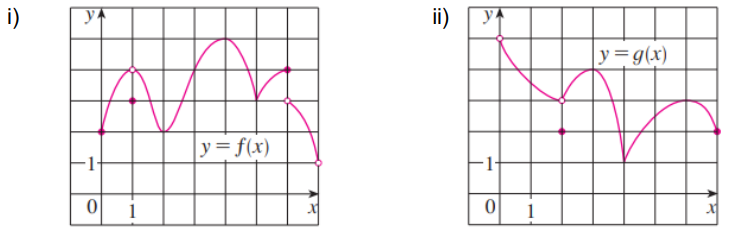
\includegraphics[width=0.85\textwidth]{./assets/graficas_ejercicio_1.png}
\end{center}

\begin{enumerate}[label=\roman*.-]

    % ----------------------------------------------------------
    % a) i)
    % ----------------------------------------------------------

    \item Para la gráfica de $f$ se observan los siguientes puntos
    relevantes:
    \[
    A=(0,2),\quad
    B=(1,3),\quad
    C=(2,2),\quad
    D=(4,5),\quad
    E=(5,3),\quad
				F=(6,4),\quad
    G=(7,1).
    \]

    El mayor valor que alcanza la función es $5$, correspondiente al
    punto $D$. Por lo tanto,

    \[
    \boxed{\text{Máximo absoluto: }D=(4,5)}
    \]

    El menor valor que alcanza la función es $2$, que se obtiene en
    los puntos $A$ y $C$. Por lo tanto,

    \[
    \boxed{
    \text{Mínimos absolutos: }
    A=(0,2),\ C=(2,2)
    }
    \]

    Los máximos locales son los puntos donde la función pasa de
    creciente a decreciente:

    \[
    \boxed{
    \text{Máximos locales: }
    D=(4,5),\ F=(6,3)
    }
    \]

    Los mínimos locales son los puntos donde la función pasa de
    decreciente a creciente:

    \[
    \boxed{
    \text{Mínimos locales: }
    B=(1,3),\ C=(2,2),\ E=(5,3)
    }
    \]


    % ----------------------------------------------------------
    % a) ii)
    % ----------------------------------------------------------

    \item El mayor valor que se aproxima a alcanzar la función es $5$, pero
    como dicho punto es abierto, la función no tiene máximo absoluto.

    \[
    \boxed{\text{Máximo absoluto: no existe}}
    \]

    El menor valor que alcanza la función es $1$, correspondiente al
    punto inferior de la gráfica:

    \[
    \boxed{\text{Mínimo absoluto: }(4,1)}
    \]

    Los máximos locales corresponden a los puntos superiores de cada
    uno de los dos arcos:

    \[
    \boxed{
    \text{Máximos locales: }(3,4),\ (6,3)
    }
    \]

    Los mínimos locales son:

    \[
    \boxed{
    \text{Mínimos locales: }(2,2),\ (4,1)
    }
    \]

\end{enumerate}

\newpage
% ============================================================
% b)
% ============================================================

\item Trace a mano la gráfica de $f$ y utilícela para encontrar los
valores máximos y mínimos, absolutos y locales, de $f$.

\begin{enumerate}[label=\roman*.-]

    % ----------------------------------------------------------
    % b) i)
    % ----------------------------------------------------------

    \item
    \[
    f(x)=\sen x,
    \qquad
    0\leq x\leq\frac{\pi}{2}.
    \]

    \begin{center}
    \begin{tikzpicture}
        \begin{axis}[
            width=9cm, height=6.5cm,
            axis lines=middle,
            xlabel={$x$}, ylabel={$f(x)$},
            xtick={0, 0.7853981634, 1.5707963268},
            xticklabels={$0$, $\pi/4$, $\pi/2$},
            ytick={0, 0.5, 1},
            xmin=-0.3, xmax=1.9,
            ymin=-0.3, ymax=1.3,
            domain=0:1.5707963268,
            samples=100,
            enlargelimits=false,
            axis line style={-Latex},
        ]
            \addplot[thick, blue, smooth] {sin(deg(x))};
            \addplot[only marks, mark=*, mark size=2pt, black]
                coordinates {(0,0) (1.5707963268,1)};
        \end{axis}
    \end{tikzpicture}
    \end{center}

    En este intervalo, la función seno es creciente. Evaluamos en los
    extremos:

    \[
    f(0)=\sen 0=0,
    \]

    \[
    f\left(\frac{\pi}{2}\right)
    =
    \sen\frac{\pi}{2}
    =1.
    \]

    Por lo tanto,

    \[
    \boxed{
    \text{Máximo absoluto: }
    \left(\frac{\pi}{2},1\right)
    }
    \]

    \[
    \boxed{
    \text{Mínimo absoluto: }(0,0)
    }
    \]

    No existen máximos ni mínimos locales en el interior del intervalo.

    \[
    \boxed{\text{Máximo local: no tiene}}
    \]

    \[
    \boxed{\text{Mínimo local: no tiene}}
    \]

				\newpage
    % ----------------------------------------------------------
    % b) ii)
    % ----------------------------------------------------------

    \item
    \[
    f(t)=\cos t,
    \qquad
    -\frac{3\pi}{2}\leq t\leq\frac{3\pi}{2}.
    \]

    \begin{center}
    \begin{tikzpicture}
        \begin{axis}[
            width=11cm, height=6.5cm,
            axis lines=middle,
            xlabel={$t$}, ylabel={$f(t)$},
            xtick={-4.7123889804, -3.1415926536, -1.5707963268, 0, 1.5707963268, 3.1415926536, 4.7123889804},
            xticklabels={$-\frac{3\pi}{2}$, $-\pi$, $-\frac{\pi}{2}$, $0$, $\frac{\pi}{2}$, $\pi$, $\frac{3\pi}{2}$},
            ytick={-1, 0, 1},
            xmin=-5.3, xmax=5.3,
            ymin=-1.4, ymax=1.4,
            domain=-4.7123889804:4.7123889804,
            samples=150,
            enlargelimits=false,
            axis line style={-Latex},
        ]
            \addplot[thick, blue, smooth] {cos(deg(x))};
            \addplot[only marks, mark=*, mark size=2pt, black]
                coordinates {(-3.1415926536,-1) (0,1) (3.1415926536,-1)};
        \end{axis}
    \end{tikzpicture}
    \end{center}

    La función alcanza su máximo cuando
    \[
    \cos t=1,
    \]
    lo cual ocurre en
    \[
    t=0.
    \]

    Por lo tanto,

    \[
    \boxed{
    \text{Máximo absoluto: }(0,1)
    }
    \]

    El valor mínimo de la función seno es $-1$, que en este intervalo
    se alcanza en
    \[
    t=-\pi
    \qquad\text{y}\qquad
    t=\pi.
    \]

    Por lo tanto,

    \[
    \boxed{
    \text{Mínimos absolutos: }
    (-\pi,-1),\ (\pi,-1)
    }
    \]

    Además,

    \[
    \boxed{\text{Máximo local: }(0,1)}
    \]

    y

    \[
    \boxed{
    \text{Mínimos locales: }
    (-\pi,-1),\ (\pi,-1)
    }
    \]

				\newpage
    % ----------------------------------------------------------
    % b) iii)
    % ----------------------------------------------------------

    \item
    \[
    f(x)=|x^2-1|.
    \]

    \begin{center}
    \begin{tikzpicture}
        \begin{axis}[
            width=10cm, height=6.5cm,
            axis lines=middle,
            xlabel={$x$}, ylabel={$f(x)$},
            xtick={-2,-1,0,1,2},
            ytick={0,1,2,3},
            xmin=-2.4, xmax=2.4,
            ymin=-0.5, ymax=3.5,
            samples=100,
            enlargelimits=false,
            axis line style={-Latex},
        ]
            \addplot[thick, blue, smooth, domain=-2.2:2.2] {abs(x^2-1)};
            \addplot[only marks, mark=*, mark size=2pt, black]
                coordinates {(-1,0) (0,1) (1,0)};
        \end{axis}
    \end{tikzpicture}
    \end{center}

    Para analizar la función podemos escribirla como

    \[
    f(x)=
    \begin{cases}
    x^2-1, & x\leq -1,\\
    1-x^2, & -1\leq x\leq1,\\
    x^2-1, & x\geq1.
    \end{cases}
    \]

    La función toma el valor $0$ cuando

    \[
    x^2-1=0,
    \]

    es decir,

    \[
    x=\pm1.
    \]

    Por lo tanto,

    \[
    f(-1)=f(1)=0.
    \]

    Como $|x^2-1|\geq0$ para todo $x$, estos puntos corresponden a
    mínimos absolutos:

    \[
    \boxed{
    \text{Mínimos absolutos: }
    (-1,0),\ (1,0)
    }
    \]

    En $x=0$ tenemos

    \[
    f(0)=1.
    \]

    Alrededor de $x=0$, la función toma valores menores que $1$,
    por lo que $(0,1)$ es un máximo local:

    \[
    \boxed{\text{Máximo local: }(0,1)}
    \]

    La función crece indefinidamente cuando $|x|\to\infty$, por lo
    que no posee máximo absoluto:

    \[
    \boxed{\text{Máximo absoluto: no existe}}
    \]

    Finalmente,

    \[
    \boxed{
    \text{Mínimos locales: }
    (-1,0),\ (1,0)
    }
    \]


    % ----------------------------------------------------------
    % b) iv)
    % ----------------------------------------------------------

    \item
    \[
    f(x)=
    \begin{cases}
    4-x^2, & -2\leq x<0,\\
    2x-1, & 0\leq x\leq2.
    \end{cases}
    \]

    \begin{center}
    \begin{tikzpicture}
        \begin{axis}[
            width=10cm, height=6.5cm,
            axis lines=middle,
            xlabel={$x$}, ylabel={$f(x)$},
            xtick={-2,-1,0,1,2},
            ytick={-1,0,1,2,3,4},
            xmin=-2.4, xmax=2.4,
            ymin=-1.5, ymax=4.5,
            samples=100,
            enlargelimits=false,
            axis line style={-Latex},
        ]
            \addplot[thick, blue, smooth, domain=-2:0, samples=80] {4-x^2};
            \addplot[thick, blue, smooth, domain=0:2, samples=80] {2*x-1};
            % puntos llenos (pertenecen a la función)
            \addplot[only marks, mark=*, mark size=2pt, black]
                coordinates {(-2,0) (0,-1) (2,3)};
            % punto vacío (no pertenece: límite del primer tramo en x=0)
            \addplot[only marks, mark=*, mark size=2pt, fill=white, draw=black]
                coordinates {(0,4)};
        \end{axis}
    \end{tikzpicture}
    \end{center}

    Analizamos cada tramo por separado.

    Para el primer tramo,

    \[
    f(x)=4-x^2,
    \qquad -2\leq x<0.
    \]

    En $x=-2$:

    \[
    f(-2)=4-(-2)^2=0.
    \]

    Cuando $x$ se aproxima a $0$ por la izquierda,

    \[
    \lim_{x\to0^-}(4-x^2)=4.
    \]

    Sin embargo, $x=0$ no pertenece al primer tramo, por lo que el
    valor $4$ no se alcanza.

    Para el segundo tramo,

    \[
    f(x)=2x-1,
    \qquad 0\leq x\leq2.
    \]

    En $x=0$:

    \[
    f(0)=2(0)-1=-1.
    \]

    En $x=2$:

    \[
    f(2)=2(2)-1=3.
    \]

    Por lo tanto, el mayor valor que se aproxima a alcanzar es $4$,
    pero dicho valor no pertenece a la función:

    \[
    \boxed{\text{Máximo absoluto: no existe}}
    \]

    El menor valor que alcanza la función es $-1$:

    \[
    \boxed{
    \text{Mínimo absoluto: }(0,-1)
    }
    \]

    Además, $(0,-1)$ es un mínimo local, ya que los valores de la
    función cercanos a $x=0$ son mayores que $-1$:

    \[
    \boxed{
    \text{Mínimo local: }(0,-1)
    }
    \]

    No existe máximo local interior en ninguno de los dos tramos.

    \[
    \boxed{\text{Máximo local: no existe}}
    \]

\end{enumerate}


% ============================================================
% c)
% ============================================================

\item Encuentre los valores máximo absoluto y mínimo absoluto de $f$
sobre el intervalo dado.

\begin{enumerate}[label=\roman*.-]

    % ----------------------------------------------------------
    % c) i)
    % ----------------------------------------------------------

    \item
    \[
    f(x)=2x^3-3x^2-12x+1,
    \qquad [-2,3].
    \]

    Calculamos la primera derivada:

    \[
    f'(x)=6x^2-6x-12.
    \]

    Factorizamos:

    \[
    f'(x)=6(x^2-x-2)
    \]

    \[
    f'(x)=6(x-2)(x+1).
    \]

    Los números críticos se obtienen de

    \[
    f'(x)=0,
    \]

    por lo que

    \[
    6(x-2)(x+1)=0.
    \]

    Entonces,

    \[
    x=-1,\qquad x=2.
    \]

    Ambos pertenecen al intervalo $[-2,3]$.

    Evaluamos la función en los extremos del intervalo y en los
    números críticos:

    \[
    f(-2)
    =
    2(-2)^3-3(-2)^2-12(-2)+1
    =
    -3,
    \]

    \[
    f(-1)
    =
    2(-1)^3-3(-1)^2-12(-1)+1
    =
    8,
    \]

    \[
    f(2)
    =
    2(2)^3-3(2)^2-12(2)+1
    =
    -19,
    \]

    \[
    f(3)
    =
    2(3)^3-3(3)^2-12(3)+1
    =
    -8.
    \]

    Comparando los valores:

    \[
    8>-3>-8>-19.
    \]

    Por lo tanto,

    \[
    \boxed{
    \text{Máximo absoluto: }(-1,8)
    }
    \]

    y

    \[
    \boxed{
    \text{Mínimo absoluto: }(2,-19)
    }.
    \]


    % ----------------------------------------------------------
    % c) ii)
    % ----------------------------------------------------------

    \item
    \[
    f(x)=\frac{x}{x^2-x+1},
    \qquad [0,3].
    \]

    Aplicamos la regla del cociente:

    \[
    f'(x)
    =
    \frac{(x^2-x+1)-x(2x-1)}
    {(x^2-x+1)^2}.
    \]

    Simplificando:

    \[
    f'(x)
    =
    \frac{1-x^2}{(x^2-x+1)^2}.
    \]

    Los números críticos se obtienen de

    \[
    1-x^2=0,
    \]

    por lo que

    \[
    x=\pm1.
    \]

    Como el intervalo es $[0,3]$, solamente consideramos

    \[
    x=1.
    \]

    Evaluamos en los extremos y en el número crítico:

    \[
    f(0)=0,
    \]

    \[
    f(1)=1,
    \]

    \[
    f(3)
    =
    \frac{3}{9-3+1}
    =
    \frac37.
    \]

    Como

    \[
    1>\frac37>0,
    \]

    obtenemos:

    \[
    \boxed{
    \text{Máximo absoluto: }(1,1)
    }
    \]

    y

    \[
    \boxed{
    \text{Mínimo absoluto: }(0,0)
    }.
    \]


    % ----------------------------------------------------------
    % c) iii)
    % ----------------------------------------------------------

    \item
    \[
    f(t)=t\sqrt{4-t^2},
    \qquad [-1,2].
    \]

    Escribimos la función como

    \[
    f(t)=t(4-t^2)^{1/2}.
    \]

    Aplicando la regla del producto:

    \[
    f'(t)
    =
    \sqrt{4-t^2}
    -
    \frac{t^2}{\sqrt{4-t^2}}.
    \]

    Llevando a común denominador:

    \[
    f'(t)
    =
    \frac{4-t^2-t^2}{\sqrt{4-t^2}},
    \]

    por lo tanto,

    \[
    \boxed{
    f'(t)=
    \frac{4-2t^2}{\sqrt{4-t^2}}
    }.
    \]

    Para encontrar los números críticos igualamos el numerador a cero:

    \[
    4-2t^2=0.
    \]

    Entonces,

    \[
    t^2=2,
    \]

    y

    \[
    t=\pm\sqrt2.
    \]

    Como el intervalo es $[-1,2]$, solamente

    \[
    t=\sqrt2
    \]

    pertenece al intervalo.

    Evaluamos en los extremos y en el número crítico:

    \[
    f(-1)
    =
    (-1)\sqrt{4-1}
    =
    -\sqrt3,
    \]

    \[
    f(\sqrt2)
    =
    \sqrt2\sqrt{4-2}
    =
    2,
    \]

    \[
    f(2)
    =
    2\sqrt{4-4}
    =
    0.
    \]

    Como

    \[
    2>0>-\sqrt3,
    \]

    tenemos:

    \[
    \boxed{
    \text{Máximo absoluto: }(\sqrt2,2)
    }
    \]

    y

    \[
    \boxed{
    \text{Mínimo absoluto: }(-1,-\sqrt3)
    }.
    \]

				\newpage
    % ----------------------------------------------------------
    % c) iv)
    % ----------------------------------------------------------

    \item
    \[
    f(t)=2\cos t+\sin 2t,
    \qquad
    \left[0,\frac{\pi}{2}\right].
    \]

    Calculamos la primera derivada:

    \[
    f'(t)=-2\sin t+2\cos2t.
    \]

    Para encontrar los números críticos:

    \[
    -2\sin t+2\cos2t=0.
    \]

    Entonces,

    \[
    \cos2t=\sin t.
    \]

    Utilizamos la identidad

    \[
    \cos2t=1-2\sin^2t.
    \]

    Por lo tanto,

    \[
    1-2\sin^2t=\sin t.
    \]

    Reordenando:

    \[
    2\sin^2t+\sin t-1=0.
    \]

    Factorizamos:

    \[
    (2\sin t-1)(\sin t+1)=0.
    \]

    De aquí:

    \[
    \sin t=\frac12
    \]

    o

    \[
    \sin t=-1.
    \]

    En el intervalo

    \[
    0\leq t\leq\frac{\pi}{2},
    \]

    solamente se cumple

    \[
    t=\frac{\pi}{6}.
    \]

    Evaluamos la función en los extremos y en el número crítico:

    \[
    f(0)
    =
    2\cos0+\sin0
    =
    2,
    \]

    \[
    f\left(\frac{\pi}{6}\right)
    =
    2\cos\frac{\pi}{6}
    +
    \sin\frac{\pi}{3}.
    \]

    Como

    \[
    \cos\frac{\pi}{6}=\frac{\sqrt3}{2}
    \]

    y

    \[
    \sin\frac{\pi}{3}=\frac{\sqrt3}{2},
    \]

    tenemos

    \[
    f\left(\frac{\pi}{6}\right)
    =
    2\left(\frac{\sqrt3}{2}\right)
    +
    \frac{\sqrt3}{2}
    =
    \frac{3\sqrt3}{2}.
    \]

    Finalmente,

    \[
    f\left(\frac{\pi}{2}\right)
    =
    2\cos\frac{\pi}{2}
    +
    \sin\pi
    =
    0.
    \]

    Como

    \[
    \frac{3\sqrt3}{2}>2>0,
    \]

    obtenemos:

    \[
    \boxed{
    \text{Máximo absoluto: }
    \left(
    \frac{\pi}{6},
    \frac{3\sqrt3}{2}
    \right)
    }
    \]

    y

    \[
    \boxed{
    \text{Mínimo absoluto: }
    \left(
    \frac{\pi}{2},
    0
    \right)
    }.
    \]

\end{enumerate}

\end{enumerate}

\volverindice
\newpage

% ======================== EJERCICIO 2 ========================

\newpage

\section{Análisis de curvas a partir de la gráfica de \texorpdfstring{$f$}{f}}

Utilice la gráfica de $f$ para encontrar lo siguiente.

\begin{center}
    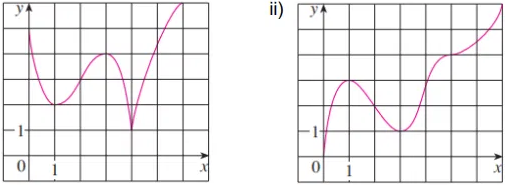
\includegraphics[width=0.85\textwidth]{./assets/graficas_ejercicio_2.png}
\end{center}

\begin{enumerate}[label=\alph*.-]

    \item Los intervalos abiertos sobre los que $f$ es creciente.

    \solucion

    \begin{itemize}
        \item \textbf{i)} $f$ es creciente en
        \[
        (1,3)\cup(4,6).
        \]

        \item \textbf{ii)} $f$ es creciente en
        \[
        (0,1)\cup(3,7).
        \]
    \end{itemize}


    \item Los intervalos abiertos sobre los que $f$ es decreciente.

    \solucion

    \begin{itemize}
        \item \textbf{i)} $f$ es decreciente en
        \[
        (0,1)\cup(3,4).
        \]

        \item \textbf{ii)} $f$ es decreciente en
        \[
        (1,3).
        \]
    \end{itemize}


    \item Los intervalos abiertos sobre los que $f$ es cóncava hacia arriba.

    \solucion

    \begin{itemize}
        \item \textbf{i)} $f$ es cóncava hacia arriba en
        \[
        (0,2).
        \]

        \item \textbf{ii)} $f$ es cóncava hacia arriba en
        \[
        (2,4)\cup(5,7).
        \]
    \end{itemize}


    \item Los intervalos abiertos sobre los que $f$ es cóncava hacia abajo.

    \solucion

    \begin{itemize}
        \item \textbf{i)} $f$ es cóncava hacia abajo en
        \[
        (2,4)\cup(4,6).
        \]

        \item \textbf{ii)} $f$ es cóncava hacia abajo en
        \[
        (0,2)\cup(4,5).
        \]
    \end{itemize}


    \item Las coordenadas de los puntos de inflexión.

    \solucion

    \begin{itemize}
        \item \textbf{i)} El punto de inflexión es
        \[
        (2,3).
        \]

        \item \textbf{ii)} Los puntos de inflexión son
        \[
        (2,2),\qquad (4,3),\qquad (5,4).
        \]
    \end{itemize}

\end{enumerate}

\volverindice

\newpage
% ======================== EJERCICIO 3 ========================

\section{Extremos locales: prueba de la primera y segunda derivada}

Encuentre los valores máximos y mínimos locales de $f$ utilizando las pruebas de la primera y la segunda derivada. ¿Qué método prefiere?

\begin{enumerate}[label=\alph*.-]

    \setcounter{enumi}{1} % comienza en b)

    \item $f(x) = \dfrac{x^2}{x - 1}$

    \solucion

    \textbf{Dominio:}

    La función no está definida en $x=1$, por lo que
    \[
    \operatorname{Dom}(f)=\mathbb{R}\setminus\{1\}.
    \]

    \textbf{1. Prueba de la primera derivada}

    Derivamos utilizando la regla del cociente:
    \[
    f'(x)
    =
    \frac{2x(x-1)-x^2}{(x-1)^2}.
    \]

    Simplificando,
    \[
    f'(x)
    =
    \frac{2x^2-2x-x^2}{(x-1)^2}
    =
    \frac{x^2-2x}{(x-1)^2}
    =
    \frac{x(x-2)}{(x-1)^2}.
    \]

    Los puntos críticos se obtienen cuando $f'(x)=0$ o cuando
    $f'(x)$ no existe, siempre que $x$ pertenezca al dominio de $f$.

    En este caso,
    \[
    x(x-2)=0,
    \]
    de donde
    \[
    x=0,\qquad x=2.
    \]

    El valor $x=1$ no es un punto crítico porque $f$ no está definida
    en dicho punto.

    Para determinar el comportamiento de la función, analizamos el signo
    de $f'(x)$:

    \[
    \begin{array}{c|ccccc}
    x & (-\infty,0) & 0 & (0,1) & (1,2) & (2,\infty)\\
    \hline
    x & - & 0 & + & + & +\\
    x-2 & - & - & - & - & +\\
    (x-1)^2 & + & + & + & + & +\\
    \hline
    f'(x) & + & 0 & - & - & +
    \end{array}
    \]

    Por lo tanto, la función es:

    \[
    \begin{cases}
    \text{creciente} & \text{en }(-\infty,0),\\
    \text{decreciente} & \text{en }(0,1)\cup(1,2),\\
    \text{creciente} & \text{en }(2,\infty).
    \end{cases}
    \]

    En $x=0$, la función pasa de creciente a decreciente. Por la
    prueba de la primera derivada, existe un \textbf{máximo local}.

    En $x=2$, la función pasa de decreciente a creciente. Por lo tanto,
    existe un \textbf{mínimo local}.

    Calculamos los valores de la función:

    \[
    f(0)=\frac{0^2}{0-1}=0,
    \]

    y

    \[
    f(2)=\frac{2^2}{2-1}=4.
    \]

    Entonces, mediante la prueba de la primera derivada:

    \[
    \boxed{\text{Máximo local: }(0,0)}
    \]

    \[
    \boxed{\text{Mínimo local: }(2,4)}
    \]

    \vspace{0.5cm}

    \textbf{2. Prueba de la segunda derivada}

    Partimos de
    \[
    f'(x)=\frac{x(x-2)}{(x-1)^2}.
    \]

    Derivamos nuevamente. Podemos escribir
    \[
    f'(x)=1-\frac{1}{(x-1)^2},
    \]
    ya que
    \[
    \frac{x^2}{x-1}=x+1+\frac{1}{x-1}.
    \]

    Por lo tanto,
    \[
    f''(x)
    =
    \frac{2}{(x-1)^3}.
    \]

    Ahora aplicamos la prueba de la segunda derivada.

    Para $x=0$:
    \[
    f''(0)
    =
    \frac{2}{(0-1)^3}
    =
    -2<0.
    \]

    Como $f''(0)<0$, la función es cóncava hacia abajo en $x=0$,
    por lo que existe un \textbf{máximo local} en ese punto.

    Para $x=2$:
    \[
    f''(2)
    =
    \frac{2}{(2-1)^3}
    =
    2>0.
    \]

    Como $f''(2)>0$, la función es cóncava hacia arriba en $x=2$,
    por lo que existe un \textbf{mínimo local} en ese punto.

    Por la prueba de la segunda derivada obtenemos nuevamente:

    \[
    \boxed{\text{Máximo local: }(0,0)}
    \]

    \[
    \boxed{\text{Mínimo local: }(2,4)}
    \]

    \textbf{Conclusión del inciso b):}

    Ambas pruebas conducen al mismo resultado. La prueba de la primera
    derivada permite observar directamente los cambios de crecimiento
    y decrecimiento, mientras que la prueba de la segunda derivada
    permite clasificar los puntos críticos de manera más rápida una vez
    calculada $f''$.


    \vspace{1cm}

    \setcounter{enumi}{3} % salta a d)

    \item $f(x) = xe^{-x^2}$

    \solucion

    \textbf{Dominio:}

    Como $e^{-x^2}$ está definida para todo número real,
    \[
    \operatorname{Dom}(f)=\mathbb{R}.
    \]

    \textbf{1. Prueba de la primera derivada}

    Utilizando la regla del producto:
    \[
    f'(x)
    =
    e^{-x^2}
    +
    x\left(-2xe^{-x^2}\right).
    \]

    Factorizando,
    \[
    f'(x)
    =
    e^{-x^2}(1-2x^2).
    \]

    Como
    \[
    e^{-x^2}>0
    \qquad \text{para todo }x\in\mathbb{R},
    \]
    los puntos críticos se obtienen de
    \[
    1-2x^2=0.
    \]

    Entonces,
    \[
    2x^2=1,
    \]
    y por lo tanto
    \[
    x^2=\frac12,
    \]
    de donde
    \[
    x=\pm\frac{1}{\sqrt2}.
    \]

    Analizamos ahora el signo de $f'(x)$. Como
    $e^{-x^2}$ siempre es positivo, el signo de $f'(x)$ depende
    únicamente de $1-2x^2$:

    \[
    \begin{array}{c|ccccc}
    x &
    (-\infty,-\frac{1}{\sqrt2}) &
    -\frac{1}{\sqrt2} &
    (-\frac{1}{\sqrt2},\frac{1}{\sqrt2}) &
    \frac{1}{\sqrt2} &
    (\frac{1}{\sqrt2},\infty)
    \\
    \hline
    f'(x) & - & 0 & + & 0 & -
    \end{array}
    \]

    Por lo tanto, la función es:

    \[
    \begin{cases}
    \text{decreciente}
    & \text{en }\left(-\infty,-\dfrac{1}{\sqrt2}\right),\\[0.3cm]
    \text{creciente}
    & \text{en }\left(-\dfrac{1}{\sqrt2},\dfrac{1}{\sqrt2}\right),\\[0.3cm]
    \text{decreciente}
    & \text{en }\left(\dfrac{1}{\sqrt2},\infty\right).
    \end{cases}
    \]

    En
    \[
    x=-\frac{1}{\sqrt2},
    \]
    la función pasa de decreciente a creciente. Por lo tanto,
    existe un \textbf{mínimo local}.

    En
    \[
    x=\frac{1}{\sqrt2},
    \]
    la función pasa de creciente a decreciente. Por lo tanto,
    existe un \textbf{máximo local}.

    Calculamos los valores correspondientes:

    \[
    f\left(-\frac{1}{\sqrt2}\right)
    =
    -\frac{1}{\sqrt2}
    e^{-\left(\frac{1}{\sqrt2}\right)^2}.
    \]

    Como
    \[
    \left(\frac{1}{\sqrt2}\right)^2=\frac12,
    \]
    resulta
    \[
    f\left(-\frac{1}{\sqrt2}\right)
    =
    -\frac{1}{\sqrt2}e^{-1/2}
    =
    -\frac{1}{\sqrt{2e}}.
    \]

    De manera análoga,
    \[
    f\left(\frac{1}{\sqrt2}\right)
    =
    \frac{1}{\sqrt2}e^{-1/2}
    =
    \frac{1}{\sqrt{2e}}.
    \]

    Entonces, mediante la prueba de la primera derivada:

    \[
    \boxed{
    \text{Mínimo local: }
    \left(-\frac{1}{\sqrt2},
    -\frac{1}{\sqrt{2e}}\right)
    }
    \]

    \[
    \boxed{
    \text{Máximo local: }
    \left(\frac{1}{\sqrt2},
    \frac{1}{\sqrt{2e}}\right)
    }
    \]

    \vspace{0.5cm}

    \textbf{2. Prueba de la segunda derivada}

    Partimos de
    \[
    f'(x)=e^{-x^2}(1-2x^2).
    \]

    Derivamos nuevamente utilizando la regla del producto:

    \[
    f''(x)
    =
    (-2xe^{-x^2})(1-2x^2)
    +
    e^{-x^2}(-4x).
    \]

    Factorizando $e^{-x^2}$:

    \[
    f''(x)
    =
    e^{-x^2}
    \left[-2x(1-2x^2)-4x\right].
    \]

    Desarrollando:

    \[
    f''(x)
    =
    e^{-x^2}
    \left(-2x+4x^3-4x\right),
    \]

    por lo que

    \[
    f''(x)
    =
    e^{-x^2}(4x^3-6x).
    \]

    Finalmente,

    \[
    \boxed{
    f''(x)=2xe^{-x^2}(2x^2-3)
    }.
    \]

    Aplicamos ahora la prueba de la segunda derivada a los puntos
    críticos.

    Para
    \[
    x=-\frac{1}{\sqrt2},
    \]
    tenemos
    \[
    2x^2-3
    =
    2\left(\frac12\right)-3
    =
    -2.
    \]

    Por lo tanto,

    \[
    f''\left(-\frac{1}{\sqrt2}\right)
    =
    2\left(-\frac{1}{\sqrt2}\right)
    e^{-1/2}(-2).
    \]

    Así,

    \[
    f''\left(-\frac{1}{\sqrt2}\right)
    =
    2\sqrt2\,e^{-1/2}>0.
    \]

    Como
    \[
    f''\left(-\frac{1}{\sqrt2}\right)>0,
    \]
    la función es cóncava hacia arriba en ese punto y, por la prueba
    de la segunda derivada, existe un \textbf{mínimo local}.

    Para
    \[
    x=\frac{1}{\sqrt2},
    \]
    nuevamente
    \[
    2x^2-3=-2.
    \]

    Entonces,

    \[
    f''\left(\frac{1}{\sqrt2}\right)
    =
    2\left(\frac{1}{\sqrt2}\right)
    e^{-1/2}(-2),
    \]

    y por lo tanto

    \[
    f''\left(\frac{1}{\sqrt2}\right)
    =
    -2\sqrt2\,e^{-1/2}<0.
    \]

    Como
    \[
    f''\left(\frac{1}{\sqrt2}\right)<0,
    \]
    la función es cóncava hacia abajo en ese punto y, por la prueba
    de la segunda derivada, existe un \textbf{máximo local}.

    Por la prueba de la segunda derivada obtenemos nuevamente:

    \[
    \boxed{
    \text{Mínimo local: }
    \left(-\frac{1}{\sqrt2},
    -\frac{1}{\sqrt{2e}}\right)
    }
    \]

    \[
    \boxed{
    \text{Máximo local: }
    \left(\frac{1}{\sqrt2},
    \frac{1}{\sqrt{2e}}\right)
    }
    \]

    \textbf{Conclusión del inciso d):}

    Ambas pruebas producen los mismos resultados. En este caso,
    la prueba de la segunda derivada resulta particularmente conveniente,
    porque una vez encontrados los puntos críticos permite clasificarlos
    evaluando directamente el signo de $f''$.

    \vspace{0.5cm}

    \textbf{Método preferido:}

    Para estos ejercicios prefiero la \textbf{prueba de la segunda
    derivada}, ya que, después de encontrar los puntos críticos, permite
    clasificarlos de forma directa: si $f''(c)>0$ hay un mínimo local y
    si $f''(c)<0$ hay un máximo local. La prueba de la primera derivada,
    sin embargo, proporciona información adicional sobre los intervalos
    de crecimiento y decrecimiento de la función.

\end{enumerate}

\volverindice
\newpage

% ======================== EJERCICIO 4 ========================

\section{Crecimiento, extremos locales y concavidad}

\begin{enumerate}[label=\alph*.-]

    \item Encuentre los intervalos sobre los cuales $f$ es creciente o decreciente.

    \item Encuentre los valores máximos y mínimos locales de $f$.

    \item Encuentre los intervalos de concavidad y los puntos de inflexión.

\end{enumerate}

\begin{enumerate}[label=\roman*.-]

    \setcounter{enumi}{1} % comienza en ii)

    \item $f(x) = \dfrac{x}{x^2 + 1}$

    \solucion

    \textbf{Dominio:}

    Como $x^2+1>0$ para todo $x\in\mathbb{R}$, la función está definida
    para todo número real:
    \[
    \operatorname{Dom}(f)=\mathbb{R}.
    \]

    \textbf{1. Crecimiento y decrecimiento}

    Calculamos la primera derivada utilizando la regla del cociente:
    \[
    f'(x)
    =
    \frac{(x^2+1)-2x^2}{(x^2+1)^2}.
    \]

    Por lo tanto,
    \[
    f'(x)=\frac{1-x^2}{(x^2+1)^2}.
    \]

    Los puntos críticos se obtienen de $f'(x)=0$:
    \[
    1-x^2=0.
    \]

    Entonces,
    \[
    x^2=1,
    \]
    de donde
    \[
    x=-1,\qquad x=1.
    \]

    Como $(x^2+1)^2>0$ para todo $x$, el signo de $f'(x)$ depende
    únicamente de $1-x^2$.

    Construimos la tabla de signos:

    \[
    \begin{array}{c|ccccc}
    x & (-\infty,-1) & -1 & (-1,1) & 1 & (1,\infty)\\
    \hline
    1-x^2 & - & 0 & + & 0 & -\\
    (x^2+1)^2 & + & + & + & + & +\\
    \hline
    f'(x) & - & 0 & + & 0 & -
    \end{array}
    \]

    Por lo tanto,
    \[
    \boxed{
    f \text{ es decreciente en }
    (-\infty,-1)\cup(1,\infty)
    }
    \]

    y
    \[
    \boxed{
    f \text{ es creciente en }(-1,1)
    }.
    \]

    \textbf{2. Máximos y mínimos locales}

    En $x=-1$, la función pasa de decreciente a creciente. Por lo tanto,
    $x=-1$ corresponde a un mínimo local.

    Calculamos su valor:
    \[
    f(-1)
    =
    \frac{-1}{(-1)^2+1}
    =
    -\frac12.
    \]

    Por lo tanto,
    \[
    \boxed{
    \text{Mínimo local: }
    \left(-1,-\frac12\right)
    }.
    \]

    En $x=1$, la función pasa de creciente a decreciente. Por lo tanto,
    $x=1$ corresponde a un máximo local.

    Calculamos su valor:
    \[
    f(1)
    =
    \frac{1}{1^2+1}
    =
    \frac12.
    \]

    Por lo tanto,
    \[
    \boxed{
    \text{Máximo local: }
    \left(1,\frac12\right)
    }.
    \]

    \textbf{3. Concavidad y puntos de inflexión}

    Partimos de
    \[
    f'(x)=\frac{1-x^2}{(x^2+1)^2}.
    \]

    Derivando nuevamente:
    \[
    f''(x)
    =
    \frac{2x(x^2-3)}{(x^2+1)^3}.
    \]

    Los posibles puntos de inflexión se obtienen de
    \[
    f''(x)=0.
    \]

    Como el denominador es siempre positivo, debemos resolver
    \[
    2x(x^2-3)=0.
    \]

    Por lo tanto,
    \[
    x=0
    \]
    o
    \[
    x^2-3=0.
    \]

    Así,
    \[
    x=-\sqrt3,\qquad x=0,\qquad x=\sqrt3.
    \]

    Construimos la tabla de signos de $f''$:

    \[
    \begin{array}{c|ccccccc}
    x &
    (-\infty,-\sqrt3) &
    -\sqrt3 &
    (-\sqrt3,0) &
    0 &
    (0,\sqrt3) &
    \sqrt3 &
    (\sqrt3,\infty)
    \\
    \hline
    x & - & - & - & 0 & + & + & +\\
    x^2-3 & + & 0 & - & - & - & 0 & +\\
    \hline
    f''(x) & - & 0 & + & 0 & - & 0 & +
    \end{array}
    \]

    Por lo tanto, $f$ es cóncava hacia abajo cuando $f''(x)<0$:

    \[
    \boxed{
    f \text{ es cóncava hacia abajo en }
    (-\infty,-\sqrt3)\cup(0,\sqrt3)
    }
    \]

    y es cóncava hacia arriba cuando $f''(x)>0$:

    \[
    \boxed{
    f \text{ es cóncava hacia arriba en }
    (-\sqrt3,0)\cup(\sqrt3,\infty)
    }.
    \]

    Como la concavidad cambia en los tres valores encontrados,
    existen tres puntos de inflexión.

    Para $x=-\sqrt3$:
    \[
    f(-\sqrt3)
    =
    \frac{-\sqrt3}{3+1}
    =
    -\frac{\sqrt3}{4}.
    \]

    Para $x=0$:
    \[
    f(0)=0.
    \]

    Para $x=\sqrt3$:
    \[
    f(\sqrt3)
    =
    \frac{\sqrt3}{3+1}
    =
    \frac{\sqrt3}{4}.
    \]

    Por lo tanto, los puntos de inflexión son

    \[
    \boxed{
    \left(-\sqrt3,-\frac{\sqrt3}{4}\right),
    \quad
    (0,0),
    \quad
    \left(\sqrt3,\frac{\sqrt3}{4}\right)
    }.
    \]

    \vspace{1cm}

				\newpage
    \setcounter{enumi}{3} % salta a iv)

    \item $f(x) = x^2\ln x$

    \solucion

    \textbf{Dominio:}

    Debido a la presencia de $\ln x$, es necesario que $x>0$.
    Por lo tanto,
    \[
    \operatorname{Dom}(f)=(0,\infty).
    \]

    \textbf{1. Crecimiento y decrecimiento}

    Calculamos la primera derivada utilizando la regla del producto:
    \[
    f'(x)
    =
    2x\ln x+x^2\frac{1}{x}.
    \]

    Simplificando:
    \[
    f'(x)=2x\ln x+x.
    \]

    Factorizamos:
    \[
    f'(x)=x(2\ln x+1).
    \]

    Los puntos críticos se obtienen de
    \[
    x(2\ln x+1)=0.
    \]

    Como $x>0$ en el dominio, $x\neq0$. Por lo tanto,
    \[
    2\ln x+1=0.
    \]

    Entonces,
    \[
    2\ln x=-1,
    \]
    \[
    \ln x=-\frac12,
    \]
    y finalmente
    \[
    x=e^{-1/2}=\frac{1}{\sqrt e}.
    \]

    Analizamos el signo de $f'(x)$. Como $x>0$, el signo depende de
    $2\ln x+1$.

    \[
    \begin{array}{c|ccc}
    x & (0,e^{-1/2}) & e^{-1/2} & (e^{-1/2},\infty)\\
    \hline
    x & + & + & +\\
    2\ln x+1 & - & 0 & +\\
    \hline
    f'(x) & - & 0 & +
    \end{array}
    \]

    Por lo tanto,
    \[
    \boxed{
    f \text{ es decreciente en }
    (0,e^{-1/2})
    }
    \]

    y
    \[
    \boxed{
    f \text{ es creciente en }
    (e^{-1/2},\infty)
    }.
    \]

    \textbf{2. Máximos y mínimos locales}

    En
    \[
    x=e^{-1/2},
    \]
    la función pasa de decreciente a creciente. Por lo tanto,
    existe un mínimo local.

    Calculamos su valor:
    \[
    f(e^{-1/2})
    =
    (e^{-1/2})^2\ln(e^{-1/2}).
    \]

    Como
    \[
    (e^{-1/2})^2=e^{-1}
    \]
    y
    \[
    \ln(e^{-1/2})=-\frac12,
    \]
    obtenemos
    \[
    f(e^{-1/2})
    =
    -\frac{1}{2e}.
    \]

    Por lo tanto,
    \[
    \boxed{
    \text{Mínimo local: }
    \left(e^{-1/2},-\frac{1}{2e}\right)
    }.
    \]

    No existe ningún máximo local, ya que la función no presenta ningún
    otro punto crítico en su dominio.

    \textbf{3. Concavidad y punto de inflexión}

    Partimos de
    \[
    f'(x)=2x\ln x+x.
    \]

    Derivando nuevamente:
    \[
    f''(x)
    =
    2\ln x+2+1.
    \]

    Por lo tanto,
    \[
    f''(x)=2\ln x+3.
    \]

    Los posibles puntos de inflexión se obtienen de
    \[
    f''(x)=0.
    \]

    Entonces,
    \[
    2\ln x+3=0,
    \]
    \[
    2\ln x=-3,
    \]
    \[
    \ln x=-\frac32.
    \]

    Por lo tanto,
    \[
    x=e^{-3/2}.
    \]

    Analizamos el signo de $f''(x)$:

    \[
    \begin{array}{c|ccc}
    x & (0,e^{-3/2}) & e^{-3/2} & (e^{-3/2},\infty)\\
    \hline
    2\ln x+3 & - & 0 & +\\
    \hline
    f''(x) & - & 0 & +
    \end{array}
    \]

    Por lo tanto, $f$ es cóncava hacia abajo en
    \[
    \boxed{
    (0,e^{-3/2})
    }
    \]

    y cóncava hacia arriba en
    \[
    \boxed{
    (e^{-3/2},\infty)
    }.
    \]

    Como la concavidad cambia de negativa a positiva en
    $x=e^{-3/2}$, existe un punto de inflexión.

    Calculamos su coordenada $y$:
    \[
    f(e^{-3/2})
    =
    (e^{-3/2})^2\ln(e^{-3/2}).
    \]

    Como
    \[
    (e^{-3/2})^2=e^{-3}
    \]
    y
    \[
    \ln(e^{-3/2})=-\frac32,
    \]
    obtenemos
    \[
    f(e^{-3/2})
    =
    -\frac{3}{2e^3}.
    \]

    Por lo tanto, el punto de inflexión es

    \[
    \boxed{
    \left(e^{-3/2},-\frac{3}{2e^3}\right)
    }.
    \]

\end{enumerate}

\volverindice
\newpage

% ======================== EJERCICIO 5 ========================

\section{Trazado de curvas}

Utilice la guía para el trazado de curvas dada en teoría para graficar cada una de las siguientes curvas.

\begin{enumerate}[label=\alph*.-]

    \setcounter{enumi}{1} % comienza en b)

    % ----------------------------------------------------------
    % b)
    % ----------------------------------------------------------

    \item $y = \dfrac{x}{x^2 + 9}$

    \solucion

    Sea
    \[
    f(x)=\frac{x}{x^2+9}.
    \]

    \textbf{A.- Dominio}

    Como
    \[
    x^2+9>0
    \qquad\text{para todo }x\in\mathbb{R},
    \]
    el denominador nunca se anula. Por lo tanto,
    \[
    \boxed{D_f=\mathbb{R}}.
    \]

    \textbf{B.- Intersecciones}

    Para encontrar la intersección con el eje $x$, hacemos $f(x)=0$:
    \[
    \frac{x}{x^2+9}=0.
    \]

    Como el denominador nunca es cero, debe cumplirse
    \[
    x=0.
    \]

    Por lo tanto, la intersección con el eje $x$ es
    \[
    (0,0).
    \]

    Para la intersección con el eje $y$, hacemos $x=0$:
    \[
    f(0)=0.
    \]

    Por lo tanto, ambas intersecciones coinciden:
    \[
    \boxed{(0,0)}.
    \]

				\newpage
    \textbf{C.- Simetría}

    Calculamos:
    \[
    f(-x)
    =
    \frac{-x}{(-x)^2+9}
    =
    -\frac{x}{x^2+9}
    =
    -f(x).
    \]

    Por lo tanto, $f$ es una función impar y su gráfica es simétrica
    respecto del origen.

    \[
    \boxed{\text{La función es impar.}}
    \]

    \textbf{D.- Asíntotas}

    No existen asíntotas verticales porque el denominador nunca se anula.

    Para determinar la asíntota horizontal calculamos:
    \[
    \lim_{x\to\pm\infty}\frac{x}{x^2+9}=0.
    \]

    Por lo tanto,
    \[
    \boxed{y=0}
    \]
    es una asíntota horizontal.

    No existe asíntota oblicua.

    \textbf{E.- Primera derivada}

    Aplicando la regla del cociente:
    \[
    f'(x)
    =
    \frac{(x^2+9)-2x^2}{(x^2+9)^2}.
    \]

    Entonces,
    \[
    f'(x)=\frac{9-x^2}{(x^2+9)^2}.
    \]

    Los números críticos se obtienen de $f'(x)=0$:
    \[
    9-x^2=0.
    \]

    Por lo tanto,
    \[
    x=-3,\qquad x=3.
    \]

    Como $(x^2+9)^2>0$, el signo de $f'(x)$ depende de $9-x^2$.

    \[
    \begin{array}{c|ccccc}
    x & (-\infty,-3) & -3 & (-3,3) & 3 & (3,\infty)\\
    \hline
    9-x^2 & - & 0 & + & 0 & -\\
    (x^2+9)^2 & + & + & + & + & +\\
    \hline
    f'(x) & - & 0 & + & 0 & -
    \end{array}
    \]

    Por lo tanto,
    \[
    \boxed{
    f\text{ es decreciente en }(-\infty,-3)\cup(3,\infty)
    }
    \]

    y
    \[
    \boxed{
    f\text{ es creciente en }(-3,3).
    }
    \]

    \textbf{F.- Valores máximos y mínimos locales}

    En $x=-3$, la función pasa de decreciente a creciente, por lo que
    existe un mínimo local.

    \[
    f(-3)=\frac{-3}{9+9}=-\frac16.
    \]

    Por lo tanto,
    \[
    \boxed{
    \text{Mínimo local: }\left(-3,-\frac16\right)
    }.
    \]

    En $x=3$, la función pasa de creciente a decreciente, por lo que
    existe un máximo local.

    \[
    f(3)=\frac{3}{9+9}=\frac16.
    \]

    Por lo tanto,
    \[
    \boxed{
    \text{Máximo local: }\left(3,\frac16\right)
    }.
    \]

    \textbf{G.- Segunda derivada, concavidad y puntos de inflexión}

    Derivamos nuevamente:
    \[
    f''(x)
    =
    \frac{2x(x^2-27)}{(x^2+9)^3}.
    \]

    Los posibles puntos de inflexión se obtienen de
    \[
    2x(x^2-27)=0.
    \]

    Por lo tanto,
    \[
    x=0,\qquad x=\pm3\sqrt3.
    \]

    Como $(x^2+9)^3>0$, el signo de $f''(x)$ depende de
    $x(x^2-27)$.

    \[
    \begin{array}{c|ccccccc}
    x &
    (-\infty,-3\sqrt3) &
    -3\sqrt3 &
    (-3\sqrt3,0) &
    0 &
    (0,3\sqrt3) &
    3\sqrt3 &
    (3\sqrt3,\infty)
    \\
    \hline
    x & - & - & - & 0 & + & + & +\\
    x^2-27 & + & 0 & - & - & - & 0 & +\\
    \hline
    f''(x) & - & 0 & + & 0 & - & 0 & +
    \end{array}
    \]

    Por lo tanto, la función es cóncava hacia abajo en
    \[
    \boxed{
    (-\infty,-3\sqrt3)\cup(0,3\sqrt3)
    }
    \]

    y cóncava hacia arriba en
    \[
    \boxed{
    (-3\sqrt3,0)\cup(3\sqrt3,\infty).
    }
    \]

    Calculamos los puntos de inflexión:

    \[
    f(-3\sqrt3)
    =
    -\frac{\sqrt3}{12},
    \]

    \[
    f(0)=0,
    \]

    \[
    f(3\sqrt3)
    =
    \frac{\sqrt3}{12}.
    \]

    Por lo tanto,
    \[
    \boxed{
    \left(-3\sqrt3,-\frac{\sqrt3}{12}\right),
    \quad
    (0,0),
    \quad
    \left(3\sqrt3,\frac{\sqrt3}{12}\right)
    }
    \]
    son los puntos de inflexión.

    \textbf{H.- Trazado de la curva}

    La gráfica es simétrica respecto del origen, pasa por $(0,0)$,
    tiene un mínimo local en $\left(-3,-\frac16\right)$ y un máximo
    local en $\left(3,\frac16\right)$, y se aproxima al eje $x$
    cuando $x\to\pm\infty$.

    \begin{center}
    \begin{tikzpicture}
    \begin{axis}[
        width=14cm, height=10cm,
        axis lines=middle,
        xlabel={$x$}, ylabel={$y$},
        xmin=-12, xmax=12, ymin=-0.3, ymax=0.3,
        xtick={-9,...,9}, ytick={-0.15,0.15},
        yticklabels={$-1/6$,$1/6$},
        grid=none,
        samples=300,
        domain=-12:12,
    ]
        % asíntota horizontal y = 0 (coincide con el eje x)
        \addplot[thick, blue] {x/(x^2+9)};
        \addplot[only marks, mark=*, mark size=1.5pt, black]
            coordinates {(-3,-0.16667) (3,0.16667) (0,0)
                         (-5.196,-0.144) (5.196,0.144)};
        \node[above right] at (axis cs:3,0.16667) {\scriptsize máx};
        \node[below right] at (axis cs:-3,-0.16667) {\scriptsize mín};
    \end{axis}
    \end{tikzpicture}
    \end{center}

    \vspace{1cm}

				\newpage
    % ----------------------------------------------------------
    % c)
    % ----------------------------------------------------------

    \item $y = \dfrac{x^3}{x^2 - 1}$

    \solucion

    Sea
    \[
    f(x)=\frac{x^3}{x^2-1}.
    \]

    \textbf{A.- Dominio}

    El denominador debe ser distinto de cero:
    \[
    x^2-1\neq0.
    \]

    Por lo tanto,
    \[
    x\neq\pm1.
    \]

    Así,
    \[
    \boxed{
    D_f=(-\infty,-1)\cup(-1,1)\cup(1,\infty)
    }.
    \]

    \textbf{B.- Intersecciones}

    Para la intersección con el eje $x$:
    \[
    \frac{x^3}{x^2-1}=0
    \quad\Longrightarrow\quad
    x=0.
    \]

    Para la intersección con el eje $y$:
    \[
    f(0)=0.
    \]

    Por lo tanto,
    \[
    \boxed{(0,0)}
    \]
    es la única intersección con ambos ejes.

    \textbf{C.- Simetría}

    Tenemos
    \[
    f(-x)
    =
    \frac{(-x)^3}{(-x)^2-1}
    =
    -\frac{x^3}{x^2-1}
    =
    -f(x).
    \]

    Por lo tanto, $f$ es impar y su gráfica es simétrica respecto
    del origen.

    \[
    \boxed{\text{La función es impar.}}
    \]

				\newpage
    \textbf{D.- Asíntotas}

    Las posibles asíntotas verticales se encuentran donde el denominador
    se anula:

    \[
    x=-1,\qquad x=1.
    \]

    Calculamos los límites laterales:

    \[
    \lim_{x\to-1^-}f(x)=-\infty,
    \qquad
    \lim_{x\to-1^+}f(x)=+\infty,
    \]

    \[
    \lim_{x\to1^-}f(x)=-\infty,
    \qquad
    \lim_{x\to1^+}f(x)=+\infty.
    \]

    Por lo tanto,
    \[
    \boxed{x=-1,\qquad x=1}
    \]
    son asíntotas verticales.

    Para encontrar la asíntota oblicua realizamos la división:
    \[
    \frac{x^3}{x^2-1}
    =
    x+\frac{x}{x^2-1}.
    \]

    Como
    \[
    \lim_{x\to\pm\infty}\frac{x}{x^2-1}=0,
    \]
    obtenemos la asíntota oblicua
    \[
    \boxed{y=x}.
    \]

    \textbf{E.- Primera derivada}

    Derivando:
    \[
    f'(x)
    =
    \frac{3x^2(x^2-1)-2x^4}{(x^2-1)^2}.
    \]

    Simplificando:
    \[
    f'(x)
    =
    \frac{x^2(x^2-3)}{(x^2-1)^2}.
    \]

    Los números críticos son
    \[
    x=0,\qquad x=\pm\sqrt3.
    \]

    Como el denominador es positivo en el dominio y $x^2\geq0$,
    el signo de $f'(x)$ depende de $x^2-3$.

    \[
    \begin{array}{c|ccccccc}
    x &
    (-\infty,-\sqrt3) &
    -\sqrt3 &
    (-\sqrt3,-1) &
    (-1,1) &
    (1,\sqrt3) &
    \sqrt3 &
    (\sqrt3,\infty)
    \\
    \hline
    x^2-3 & + & 0 & - & - & - & 0 & +\\
    \hline
    f'(x) & + & 0 & - & - & - & 0 & +
    \end{array}
    \]

    El punto $x=0$ también es crítico, pero el signo de $f'$ es
    negativo a ambos lados, por lo que no constituye un extremo local.

    Así,
    \[
    \boxed{
    f\text{ es creciente en }
    (-\infty,-\sqrt3)\cup(\sqrt3,\infty)
    }
    \]

    y
    \[
    \boxed{
    f\text{ es decreciente en }
    (-\sqrt3,-1)\cup(-1,1)\cup(1,\sqrt3).
    }
    \]

    \textbf{F.- Valores máximos y mínimos locales}

    En $x=-\sqrt3$, $f'$ cambia de positivo a negativo. Por lo tanto,
    existe un máximo local:

    \[
    f(-\sqrt3)
    =
    \frac{-3\sqrt3}{2}.
    \]

    Así,
    \[
    \boxed{
    \text{Máximo local: }
    \left(-\sqrt3,-\frac{3\sqrt3}{2}\right)
    }.
    \]

    En $x=\sqrt3$, $f'$ cambia de negativo a positivo. Por lo tanto,
    existe un mínimo local:

    \[
    f(\sqrt3)
    =
    \frac{3\sqrt3}{2}.
    \]

    Entonces,
    \[
    \boxed{
    \text{Mínimo local: }
    \left(\sqrt3,\frac{3\sqrt3}{2}\right)
    }.
    \]

    \textbf{G.- Segunda derivada, concavidad y puntos de inflexión}

    Derivando nuevamente:
    \[
    f''(x)
    =
    \frac{2x(x^2+3)}{(x^2-1)^3}.
    \]

    Como $x^2+3>0$, el signo depende de
    \[
    \frac{x}{(x^2-1)^3}.
    \]

    \[
    \begin{array}{c|ccccc}
    x & (-\infty,-1) & (-1,0) & 0 & (0,1) & (1,\infty)\\
    \hline
    x & - & - & 0 & + & +\\
    (x^2-1)^3 & + & - & - & - & +\\
    \hline
    f''(x) & - & + & 0 & - & +
    \end{array}
    \]

    Por lo tanto, $f$ es cóncava hacia abajo en
    \[
    \boxed{
    (-\infty,-1)\cup(0,1)
    }
    \]

    y cóncava hacia arriba en
    \[
    \boxed{
    (-1,0)\cup(1,\infty).
    }
    \]

    El único valor del dominio donde $f''(x)=0$ es $x=0$ y allí
    cambia la concavidad. Por lo tanto,
    \[
    f(0)=0
    \]
    y el único punto de inflexión es
    \[
    \boxed{(0,0)}.
    \]

    \textbf{H.- Trazado de la curva}

    La gráfica es simétrica respecto del origen, posee asíntotas
    verticales $x=-1$ y $x=1$, y asíntota oblicua $y=x$.
    Presenta un máximo local en
    $\left(-\sqrt3,-\frac{3\sqrt3}{2}\right)$ y un mínimo local en
    $\left(\sqrt3,\frac{3\sqrt3}{2}\right)$.

    \begin{center}
    \begin{tikzpicture}
    \begin{axis}[
        width=14cm, height=12cm,
        axis lines=middle,
        xlabel={$x$}, ylabel={$y$},
        xmin=-5, xmax=5, ymin=-6, ymax=6,
        grid=none,
        samples=200,
        restrict y to domain=-6:6,
    ]
        % asíntota oblicua y = x
        \addplot[dashed, gray, domain=-5:5] {x};
        % asíntotas verticales x = -1, x = 1
        \addplot[dashed, gray] coordinates {(-1,-6) (-1,6)};
        \addplot[dashed, gray] coordinates {(1,-6) (1,6)};
        % ramas de la función en cada subintervalo del dominio
        \addplot[thick, blue, domain=-5:-1.05] {x^3/(x^2-1)};
        \addplot[thick, blue, domain=-0.95:0.95] {x^3/(x^2-1)};
        \addplot[thick, blue, domain=1.05:5] {x^3/(x^2-1)};
        \addplot[only marks, mark=*, mark size=1.5pt, black]
            coordinates {(-1.732,-2.598) (1.732,2.598) (0,0)};
        \node[above left] at (axis cs:-1.732,-2.598) {\scriptsize máx};
        \node[below right] at (axis cs:1.732,2.598) {\scriptsize mín};
    \end{axis}
    \end{tikzpicture}
    \end{center}

    \vspace{1cm}

				\newpage
    % ----------------------------------------------------------
    % f)
    % ----------------------------------------------------------

    \setcounter{enumi}{5} % salta a f)

    \item $y = \dfrac{e^x}{x^2}$

    \solucion

    Sea
    \[
    f(x)=\frac{e^x}{x^2}.
    \]

    \textbf{A.- Dominio}

    Como $x^2\neq0$ cuando $x\neq0$,
    \[
    \boxed{D_f=(-\infty,0)\cup(0,\infty)}.
    \]

    \textbf{B.- Intersecciones}

    Para todo $x$,
    \[
    e^x>0.
    \]

    Por lo tanto,
    \[
    \frac{e^x}{x^2}>0
    \]
    para todo $x$ del dominio.

    La función no corta al eje $x$ y tampoco está definida en $x=0$.

    \[
    \boxed{\text{No posee intersecciones con los ejes.}}
    \]

    \textbf{C.- Simetría}

    Tenemos
    \[
    f(-x)=\frac{e^{-x}}{x^2},
    \]
    que no es igual ni a $f(x)$ ni a $-f(x)$.

    Por lo tanto,
    \[
    \boxed{\text{La función no es par ni impar.}}
    \]

    \textbf{D.- Asíntotas}

    Como
    \[
    \lim_{x\to0^-}\frac{e^x}{x^2}=+\infty
    \]
    y
    \[
    \lim_{x\to0^+}\frac{e^x}{x^2}=+\infty,
    \]
    tenemos la asíntota vertical
    \[
    \boxed{x=0}.
    \]

    Para $x\to-\infty$:
    \[
    \lim_{x\to-\infty}\frac{e^x}{x^2}=0.
    \]

    Por lo tanto,
    \[
    \boxed{y=0}
    \]
    es una asíntota horizontal hacia la izquierda.

    Para $x\to+\infty$,
    \[
    \lim_{x\to+\infty}\frac{e^x}{x^2}=+\infty,
    \]
    por lo que no existe asíntota horizontal hacia la derecha.

    \textbf{E.- Primera derivada}

    Escribimos
    \[
    f(x)=e^x x^{-2}.
    \]

    Entonces,
    \[
    f'(x)
    =
    e^x x^{-2}-2e^x x^{-3}.
    \]

    Por lo tanto,
    \[
    f'(x)
    =
    \frac{e^x(x-2)}{x^3}.
    \]

    Como $e^x>0$, analizamos el signo de
    $(x-2)/x^3$.

    El único número crítico es
    \[
    x=2.
    \]

    \[
    \begin{array}{c|ccc}
    x & (-\infty,0) & (0,2) & (2,\infty)\\
    \hline
    x-2 & - & - & +\\
    x^3 & - & + & +\\
    \hline
    f'(x) & + & - & +
    \end{array}
    \]

    Por lo tanto,
    \[
    \boxed{
    f\text{ es creciente en }(-\infty,0)\cup(2,\infty)
    }
    \]

    y
    \[
    \boxed{
    f\text{ es decreciente en }(0,2).
    }
    \]

    \textbf{F.- Valores máximos y mínimos locales}

    En $x=2$, la función pasa de decreciente a creciente. Por lo tanto,
    existe un mínimo local.

    \[
    f(2)=\frac{e^2}{4}.
    \]

    Así,
    \[
    \boxed{
    \text{Mínimo local: }\left(2,\frac{e^2}{4}\right)
    }.
    \]

    No existe máximo local.

    \textbf{G.- Segunda derivada, concavidad y puntos de inflexión}

    Derivando nuevamente:
    \[
    f''(x)
    =
    \frac{e^x(x^2-4x+6)}{x^4}.
    \]

    Observamos que
    \[
    x^2-4x+6
    =
    (x-2)^2+2>0.
    \]

    Además,
    \[
    e^x>0,\qquad x^4>0.
    \]

    Por lo tanto,
    \[
    \boxed{f''(x)>0}
    \]
    para todo $x$ del dominio.

    Así, la función es cóncava hacia arriba en
    \[
    \boxed{(-\infty,0)\cup(0,\infty)}.
    \]

    Como $f''(x)$ nunca se anula y $x=0$ no pertenece al dominio,
    no existen puntos de inflexión.

    \[
    \boxed{\text{No hay puntos de inflexión.}}
    \]

    \textbf{H.- Trazado de la curva}

    La función es siempre positiva, tiene una asíntota vertical $x=0$,
    se aproxima al eje $x$ cuando $x\to-\infty$, alcanza un mínimo local
    en $\left(2,\frac{e^2}{4}\right)$ y es cóncava hacia arriba en todo
    su dominio.

    \begin{center}
    \begin{tikzpicture}
    \begin{axis}[
        width=10cm, height=7cm,
        axis lines=middle,
        xlabel={$x$}, ylabel={$y$},
        xmin=-5, xmax=3.5, ymin=-0.5, ymax=6,
        grid=none,
        samples=200,
        restrict y to domain=-1:6,
    ]
        % asíntota vertical x = 0
        \addplot[dashed, gray] coordinates {(0,-0.5) (0,6)};
        % ramas de la función
        \addplot[thick, blue, domain=-5:-0.1] {exp(x)/x^2};
        \addplot[thick, blue, domain=0.1:3.3] {exp(x)/x^2};
        \addplot[only marks, mark=*, mark size=1.5pt, black]
            coordinates {(2,1.847)};
        \node[below right] at (axis cs:2,1.847) {\scriptsize mín};
    \end{axis}
    \end{tikzpicture}
    \end{center}


    \vspace{1cm}

% ----------------------------------------------------------
% h)
% ----------------------------------------------------------

\setcounter{enumi}{7} % salta a h)

\item $y = xe^{-1/x}$

\solucion

Sea

\[
f(x)=xe^{-1/x}.
\]

\textbf{A.- Dominio}

Debido a la expresión $-1/x$, debemos tener

\[
x\neq0.
\]

Por lo tanto,

\[
\boxed{
D_f=(-\infty,0)\cup(0,\infty)
}.
\]

\textbf{B.- Intersecciones}

Para que $f(x)=0$:

\[
xe^{-1/x}=0.
\]

Como la función exponencial nunca es cero, esto exigiría

\[
x=0,
\]

pero $x=0$ no pertenece al dominio.

Por lo tanto,

\[
\boxed{\text{La función no posee intersecciones con los ejes.}}
\]

\textbf{C.- Simetría}

Calculamos:

\[
f(-x)
=
(-x)e^{-1/(-x)}
=
-xe^{1/x}.
\]

Esto no coincide ni con $f(x)$ ni con $-f(x)$.

Por lo tanto,

\[
\boxed{\text{La función no es par ni impar.}}
\]

\textbf{D.- Asíntotas}

Para $x\to0^+$:

\[
\lim_{x\to0^+}xe^{-1/x}=0.
\]

Para $x\to0^-$:

\[
\lim_{x\to0^-}xe^{-1/x}=-\infty.
\]

Por lo tanto,

\[
\boxed{x=0}
\]

es una asíntota vertical, ya que al menos uno de los
límites laterales es infinito.

Para determinar las asíntotas oblicuas, calculamos

\[
m=
\lim_{x\to\pm\infty}
\frac{f(x)}{x}.
\]

Entonces,

\[
m=
\lim_{x\to\pm\infty}
\frac{xe^{-1/x}}{x}
=
\lim_{x\to\pm\infty}
e^{-1/x}
=
1.
\]

Ahora calculamos

\[
b=
\lim_{x\to\pm\infty}
\left[f(x)-mx\right].
\]

Como $m=1$:

\[
b=
\lim_{x\to\pm\infty}
\left(xe^{-1/x}-x\right).
\]

Factorizando $x$:

\[
b=
\lim_{x\to\pm\infty}
x\left(e^{-1/x}-1\right).
\]

Hacemos el cambio de variable

\[
u=-\frac{1}{x}.
\]

Cuando $x\to\pm\infty$, se tiene $u\to0$, y además

\[
x=-\frac{1}{u}.
\]

Por lo tanto,

\[
b=
\lim_{u\to0}
-\frac{e^u-1}{u}.
\]

Como

\[
\lim_{u\to0}
\frac{e^u-1}{u}=1,
\]

obtenemos

\[
b=-1.
\]

Por lo tanto,

\[
\boxed{y=x-1}
\]

es una asíntota oblicua tanto para $x\to+\infty$
como para $x\to-\infty$.

    \textbf{E.- Primera derivada}

    Utilizando la regla del producto:
    \[
    f'(x)
    =
    e^{-1/x}
    +
    x e^{-1/x}\frac{1}{x^2}.
    \]

    Por lo tanto,
    \[
    f'(x)
    =
    e^{-1/x}\left(1+\frac1x\right)
    =
    \frac{(x+1)e^{-1/x}}{x}.
    \]

    Como $e^{-1/x}>0$, el signo depende de
    \[
    \frac{x+1}{x}.
    \]

    El único número crítico es
    \[
    x=-1.
    \]

\[
\begin{array}{c|cccc}
x & (-\infty,-1) & -1 & (-1,0) & (0,\infty)\\
\hline
x+1 & - & 0 & + & +\\
x & - & - & - & +\\
\hline
f'(x) & + & 0 & - & +
\end{array}
\]

    Por lo tanto,
    \[
    \boxed{
    f\text{ es creciente en }(-\infty,-1)\cup(0,\infty)
    }
    \]

    y
    \[
    \boxed{
    f\text{ es decreciente en }(-1,0).
    }
    \]

    \textbf{F.- Valores máximos y mínimos locales}

    En $x=-1$, la función pasa de creciente a decreciente. Por lo tanto,
    existe un máximo local.

    \[
    f(-1)
    =
    -1\cdot e^{-1/(-1)}
    =
    -e.
    \]

    Así,
    \[
    \boxed{
    \text{Máximo local: }(-1,-e)
    }.
    \]

    No existe mínimo local.

    \textbf{G.- Segunda derivada, concavidad y puntos de inflexión}

    Derivando nuevamente:
    \[
    f''(x)=\frac{e^{-1/x}}{x^3}.
    \]

    Como la exponencial es siempre positiva, el signo depende de $x^3$:

    \[
    \begin{array}{c|cc}
    x & (-\infty,0) & (0,\infty)\\
    \hline
    x^3 & - & +\\
    \hline
    f''(x) & - & +
    \end{array}
    \]

    Por lo tanto,
    \[
    \boxed{
    f\text{ es cóncava hacia abajo en }(-\infty,0)
    }
    \]

    y
    \[
    \boxed{
    f\text{ es cóncava hacia arriba en }(0,\infty).
    }
    \]

    Aunque la concavidad cambia al pasar por $x=0$, este punto no
    pertenece al dominio. Por lo tanto, $x=0$ no puede ser un punto
    de inflexión.

    \[
    \boxed{\text{No existen puntos de inflexión.}}
    \]

    \textbf{H.- Trazado de la curva}

    La gráfica tiene asíntota vertical $x=0$ y asíntota oblicua
    $y=x-1$. Posee un máximo local en $(-1,-e)$, es cóncava hacia abajo
    en el semieje negativo y cóncava hacia arriba en el semieje positivo.

    \begin{center}
    \begin{tikzpicture}
    \begin{axis}[
        width=10cm, height=8cm,
        axis lines=middle,
        xlabel={$x$}, ylabel={$y$},
        xmin=-5, xmax=5, ymin=-6, ymax=5,
        grid=none,
        samples=200,
        restrict y to domain=-6:5,
    ]
        % asíntota oblicua y = x - 1
        \addplot[dashed, gray, domain=-5:5] {x-1};
        % asíntota vertical x = 0
        \addplot[dashed, gray] coordinates {(0,-6) (0,5)};
        % ramas de la función
        \addplot[thick, blue, domain=-5:-0.05] {x*exp(-1/x)};
        \addplot[thick, blue, domain=0.09:5] {x*exp(-1/x)};
        \addplot[only marks, mark=*, mark size=1.5pt, black]
            coordinates {(-1,-2.718)};
        \node[below left] at (axis cs:-1,-2.718) {\scriptsize máx};
    \end{axis}
    \end{tikzpicture}
    \end{center}


    \vspace{1cm}

    % ----------------------------------------------------------
    % último ejercicio
    % ----------------------------------------------------------

    \item $y = \dfrac{\ln x}{x^2}$

    \solucion

    Sea
    \[
    f(x)=\frac{\ln x}{x^2}.
    \]

    \textbf{A.- Dominio}

    Como $\ln x$ está definido solamente para $x>0$,
    \[
    \boxed{D_f=(0,\infty)}.
    \]

    \textbf{B.- Intersecciones}

    Para encontrar la intersección con el eje $x$:
    \[
    \frac{\ln x}{x^2}=0.
    \]

    Como $x^2>0$, debe cumplirse
    \[
    \ln x=0,
    \]
    de donde
    \[
    x=1.
    \]

    Por lo tanto,
    \[
    \boxed{(1,0)}
    \]
    es la intersección con el eje $x$.

    No existe intersección con el eje $y$ porque $x=0$ no pertenece
    al dominio.

				\newpage
    \textbf{C.- Simetría}

    La función no puede ser par ni impar porque su dominio no es
    simétrico respecto del origen.

    \[
    \boxed{\text{La función no es par ni impar.}}
    \]

    \textbf{D.- Asíntotas}

    Para $x\to0^+$:
    \[
    \lim_{x\to0^+}\frac{\ln x}{x^2}=-\infty.
    \]

    Por lo tanto,
    \[
    \boxed{x=0}
    \]
    es una asíntota vertical.

    Para $x\to+\infty$:
    \[
    \lim_{x\to+\infty}\frac{\ln x}{x^2}=0.
    \]

    Por lo tanto,
    \[
    \boxed{y=0}
    \]
    es una asíntota horizontal.

    \textbf{E.- Primera derivada}

    Escribimos
    \[
    f(x)=(\ln x)x^{-2}.
    \]

    Entonces,
    \[
    f'(x)
    =
    \frac1x x^{-2}
    -2(\ln x)x^{-3}.
    \]

    Por lo tanto,
    \[
    f'(x)
    =
    \frac{1-2\ln x}{x^3}.
    \]

    Los números críticos se obtienen de
    \[
    1-2\ln x=0.
    \]

    Entonces,
    \[
    \ln x=\frac12,
    \]
    y por lo tanto
    \[
    x=e^{1/2}=\sqrt e.
    \]

    Como $x^3>0$ para $x>0$, el signo de $f'(x)$ depende de
    $1-2\ln x$.

    \[
    \begin{array}{c|ccc}
    x & (0,\sqrt e) & \sqrt e & (\sqrt e,\infty)\\
    \hline
    1-2\ln x & + & 0 & -\\
    x^3 & + & + & +\\
    \hline
    f'(x) & + & 0 & -
    \end{array}
    \]

    Por lo tanto,
    \[
    \boxed{
    f\text{ es creciente en }(0,\sqrt e)
    }
    \]

    y
    \[
    \boxed{
    f\text{ es decreciente en }(\sqrt e,\infty).
    }
    \]

    \textbf{F.- Valores máximos y mínimos locales}

    En $x=\sqrt e$, la función pasa de creciente a decreciente.
    Por lo tanto, existe un máximo local.

    \[
    f(\sqrt e)
    =
    \frac{\ln(\sqrt e)}{(\sqrt e)^2}.
    \]

    Como
    \[
    \ln(\sqrt e)=\frac12
    \]
    y
    \[
    (\sqrt e)^2=e,
    \]
    obtenemos
    \[
    f(\sqrt e)=\frac{1}{2e}.
    \]

    Por lo tanto,
    \[
    \boxed{
    \text{Máximo local: }
    \left(\sqrt e,\frac{1}{2e}\right)
    }.
    \]

    No existe mínimo local.

    \textbf{G.- Segunda derivada, concavidad y punto de inflexión}

    Derivando nuevamente:
    \[
    f''(x)
    =
    \frac{6\ln x-5}{x^4}.
    \]

    Como $x^4>0$ para todo $x>0$, el signo depende de
    \[
    6\ln x-5.
    \]

    Los posibles puntos de inflexión se obtienen de
    \[
    6\ln x-5=0.
    \]

    Entonces,
    \[
    \ln x=\frac56,
    \]
    por lo que
    \[
    x=e^{5/6}.
    \]

    Construimos la tabla de signos:

    \[
    \begin{array}{c|ccc}
    x & (0,e^{5/6}) & e^{5/6} & (e^{5/6},\infty)\\
    \hline
    6\ln x-5 & - & 0 & +\\
    x^4 & + & + & +\\
    \hline
    f''(x) & - & 0 & +
    \end{array}
    \]

    Por lo tanto,
    \[
    \boxed{
    f\text{ es cóncava hacia abajo en }(0,e^{5/6})
    }
    \]

    y
    \[
    \boxed{
    f\text{ es cóncava hacia arriba en }(e^{5/6},\infty).
    }
    \]

    Como la concavidad cambia en $x=e^{5/6}$, existe un punto
    de inflexión.

    Calculamos su coordenada $y$:

    \[
    f(e^{5/6})
    =
    \frac{\ln(e^{5/6})}{(e^{5/6})^2}.
    \]

    Entonces,
    \[
    f(e^{5/6})
    =
    \frac{5/6}{e^{5/3}}
    =
    \frac{5}{6e^{5/3}}.
    \]

    Por lo tanto, el punto de inflexión es

    \[
    \boxed{
    \left(e^{5/6},\frac{5}{6e^{5/3}}\right)
    }.
    \]

    \textbf{H.- Trazado de la curva}

    La gráfica está definida solamente para $x>0$, posee una asíntota
    vertical $x=0$ y una asíntota horizontal $y=0$. Corta al eje $x$
    en $(1,0)$, alcanza un máximo local en
    $\left(\sqrt e,\frac{1}{2e}\right)$ y cambia de concavidad en
    $\left(e^{5/6},\frac{5}{6e^{5/3}}\right)$.

    \begin{center}

\begin{tikzpicture}

\begin{axis}[
    width=10cm,
    height=7cm,
    axis lines=middle,
    xlabel={$x$},
    ylabel={$y$},
    xmin=-0.5,
    xmax=8,
    ymin=-1.5,
    ymax=0.3,
    grid=none,
    samples=300,
    restrict y to domain=-1.5:0.3,
]
    \addplot[
        dashed,
        gray
    ] coordinates {(0,-1.5) (0,0.3)};
    \addplot[
        dashed,
        gray
    ] coordinates {(0,0) (8,0)};
    \addplot[
        thick,
        blue,
        domain=0.05:8
    ] {ln(x)/x^2};
    \addplot[
        only marks,
        mark=*,
        mark size=1.5pt,
        black
    ]
    coordinates {
        (1,0)
        (1.6487,0.1839)
        (2.301,0.1574)
    };
    \node[
        above right
    ]
    at (axis cs:1.6487,0.1839)
    {\scriptsize máx};
    \node[
        below right
    ]
    at (axis cs:2.301,0.1574)
    {\scriptsize infl.};
    \node[
        above left
    ]
    at (axis cs:0,0.25)
    {\scriptsize $x=0$};
\end{axis}
\end{tikzpicture}
\end{center}
\end{enumerate}

\volverindice
\newpage

% ======================== EJERCICIO 6 ========================

\section{Optimización: planteo de la función a optimizar}

Indique la función, de una variable, a optimizar en los siguientes casos:

\begin{enumerate}[label=\alph*.-]

    \setcounter{enumi}{1} % comienza en b)

    % ----------------------------------------------------------
    % b)
    % ----------------------------------------------------------

    \item Encuentre el punto sobre la recta $y = 2x + 3$ que está más cerca del origen.

    \solucion

    Sea $P=(x,y)$ un punto cualquiera de la recta
    \[
    y=2x+3.
    \]

    La distancia desde el origen $O=(0,0)$ hasta el punto $P=(x,y)$
    está dada por
    \[
    d=\sqrt{x^2+y^2}.
    \]

    Como $y=2x+3$, podemos expresar la distancia únicamente en función
    de $x$:
    \[
    d(x)=\sqrt{x^2+(2x+3)^2}.
    \]

    Para simplificar el proceso de optimización, podemos minimizar el
    cuadrado de la distancia, ya que la función raíz cuadrada es
    creciente. Por lo tanto, la función a optimizar es
    \[
    D(x)=x^2+(2x+3)^2.
    \]

    Desarrollando:
    \[
    D(x)=x^2+4x^2+12x+9,
    \]
    \[
    \boxed{D(x)=5x^2+12x+9}.
    \]

    Por lo tanto, la función de una variable a minimizar es
    \[
    \boxed{D(x)=5x^2+12x+9},
    \qquad x\in\mathbb{R}.
    \]

    Una vez encontrado el valor de $x$, la coordenada $y$ se obtiene
    mediante
    \[
    y=2x+3.
    \]


    \vspace{1cm}

				\newpage
    % ----------------------------------------------------------
    % c)
    % ----------------------------------------------------------

    \item Encuentre las dimensiones de un rectángulo con área de
    $1000 \text{ m}^2$ cuyo perímetro sea tan pequeño como sea posible.

    \solucion

    Sean $x$ e $y$ las dimensiones del rectángulo.

    La condición del área es
    \[
    xy=1000.
    \]

    Despejamos $y$:
    \[
    y=\frac{1000}{x}.
    \]

    El perímetro del rectángulo es
    \[
    P=2x+2y.
    \]

    Sustituyendo $y$:
    \[
    P(x)=2x+2\left(\frac{1000}{x}\right).
    \]

    Por lo tanto, la función de una variable que debemos minimizar es
    \[
    \boxed{
    P(x)=2x+\frac{2000}{x}
    },
    \qquad x>0.
    \]

    Una vez obtenido el valor óptimo de $x$, la otra dimensión se
    obtiene mediante
    \[
    y=\frac{1000}{x}.
    \]


    \vspace{1cm}

				\newpage
    % ----------------------------------------------------------
    % d)
    % ----------------------------------------------------------

    \item Si se dispone de $1200 \text{ cm}^2$ de material para hacer
    una caja con una base cuadrada y sin tapa; encuentre el mayor
    volumen posible de la caja.

    \solucion

    Sea $x$ el lado de la base cuadrada y sea $h$ la altura de la caja.

    Como la caja no tiene tapa, el área de material utilizada está
    formada por el área de la base y las cuatro caras laterales:
    \[
    x^2+4xh=1200.
    \]

    Despejamos $h$:
    \[
    4xh=1200-x^2,
    \]
    \[
    h=\frac{1200-x^2}{4x}.
    \]

    El volumen de la caja es
    \[
    V=x^2h.
    \]

    Sustituyendo la expresión obtenida para $h$:
    \[
    V(x)
    =
    x^2\left(\frac{1200-x^2}{4x}\right).
    \]

    Simplificando:
    \[
    V(x)
    =
    \frac{x(1200-x^2)}{4}.
    \]

    Por lo tanto,
    \[
    \boxed{
    V(x)=300x-\frac{x^3}{4}
    }.
    \]

    Como $x>0$ y además debe cumplirse $h>0$, tenemos
    \[
    1200-x^2>0,
    \]
    de donde
    \[
    0<x<20\sqrt3.
    \]

    Por lo tanto, la función de una variable que debemos maximizar es
    \[
    \boxed{
    V(x)=300x-\frac{x^3}{4},
    \qquad 0<x<20\sqrt3.
    }
    \]

\end{enumerate}

\volverindice
\newpage

% ======================== EJERCICIO 7 ========================
\section{Situaciones problemáticas de optimización}

Resuelva las siguientes situaciones problemáticas:

\begin{enumerate}[label=\alph*.-]

    \setcounter{enumi}{2} % comienza en c)

    % ----------------------------------------------------------
    % c)
    % ----------------------------------------------------------

    \item Una caja con una base cuadrada, abierta en la parte superior,
    debe tener un volumen de $32.000 \text{ cm}^3$. Encuentre las
    dimensiones de la caja que minimicen la cantidad de material que
    ha de utilizarse.

    \solucion

    Sea $x$ el lado de la base cuadrada y $h$ la altura de la caja.

    Como la caja está abierta en la parte superior, el material utilizado
    corresponde al área de la base más el área de las cuatro caras
    laterales.

    El volumen de la caja debe ser
    \[
    V=x^2h=32.000.
    \]

    Despejamos $h$:
    \[
    h=\frac{32.000}{x^2}.
    \]

    La cantidad de material utilizada es el área de superficie de la
    caja:
    \[
    S=x^2+4xh.
    \]

    Sustituyendo la expresión obtenida para $h$:
    \[
    S(x)
    =
    x^2+4x\left(\frac{32.000}{x^2}\right).
    \]

    Simplificando:
    \[
    S(x)=x^2+\frac{128.000}{x}.
    \]

    Por lo tanto, debemos minimizar
    \[
    \boxed{
    S(x)=x^2+\frac{128.000}{x}
    },
    \qquad x>0.
    \]

    \textbf{Primera derivada}

    Derivamos:
    \[
    S'(x)=2x-\frac{128.000}{x^2}.
    \]

    Buscamos los números críticos:
    \[
    2x-\frac{128.000}{x^2}=0.
    \]

    Multiplicando por $x^2$:
    \[
    2x^3-128.000=0.
    \]

    Entonces,
    \[
    2x^3=128.000,
    \]
    \[
    x^3=64.000,
    \]
    y por lo tanto
    \[
    x=40.
    \]

    Como $x>0$, este es el único número crítico del dominio.

    Para determinar el comportamiento de $S$, analizamos el signo de
    $S'(x)$:

    \[
    \begin{array}{c|ccc}
    x & (0,40) & 40 & (40,\infty)\\
    \hline
    2x^3-128.000 & - & 0 & +\\
    x^2 & + & + & +\\
    \hline
    S'(x) & - & 0 & +
    \end{array}
    \]

    Por lo tanto, $S(x)$ es decreciente en $(0,40)$ y creciente en
    $(40,\infty)$. En consecuencia, en $x=40$ se alcanza un mínimo.

    \textbf{Comprobación mediante la segunda derivada}

    Calculamos:
    \[
    S''(x)=2+\frac{256.000}{x^3}.
    \]

    Como $x>0$,
    \[
    S''(x)>0.
    \]

    En particular,
    \[
    S''(40)>0,
    \]
    por lo que $x=40$ corresponde a un mínimo.

    \textbf{Altura de la caja}

    Utilizando
    \[
    h=\frac{32.000}{x^2},
    \]
    obtenemos
    \[
    h=\frac{32.000}{40^2}
    =
    \frac{32.000}{1.600}
    =
    20.
    \]

    Por lo tanto, las dimensiones de la caja que minimizan la cantidad
    de material son

    \[
    \boxed{
    40\text{ cm}\times40\text{ cm}\times20\text{ cm}
    }.
    \]

    Es decir, la base es un cuadrado de lado $40$ cm y la altura es
    $20$ cm.


    \vspace{1cm}

    % ----------------------------------------------------------
    % d)
    % ----------------------------------------------------------

    \item Se desea construir una caja con tapa abierta, utilizando una
    pieza cuadrada de cartón de 3 pies de ancho, recortando un cuadrado
    en cada una de las cuatro esquinas y doblando los costados.
    Encuentre el volumen más grande que esa caja puede tener.

    \solucion

    Sea $x$ el lado de cada uno de los cuadrados que se recortan
    en las cuatro esquinas.

    Al realizar los cortes y doblar los lados, la altura de la caja
    será
    \[
    h=x.
    \]

    Como la pieza original de cartón tiene $3$ pies de lado, las
    dimensiones de la base de la caja serán
    \[
    3-2x
    \]
    por
    \[
    3-2x.
    \]

    Por lo tanto, el volumen de la caja es
    \[
    V=x(3-2x)^2.
    \]

    Para que la caja tenga dimensiones positivas debe cumplirse
    \[
    x>0
    \]
    y
    \[
    3-2x>0.
    \]

    De donde
    \[
    0<x<\frac32.
    \]

    Por lo tanto, debemos maximizar
    \[
    \boxed{
    V(x)=x(3-2x)^2,
    \qquad 0<x<\frac32.
    }
    \]

    Desarrollando:
    \[
    V(x)
    =
    x(9-12x+4x^2),
    \]
    \[
    V(x)=9x-12x^2+4x^3.
    \]

    \textbf{Primera derivada}

    Derivamos:
    \[
    V'(x)=9-24x+12x^2.
    \]

    Buscamos los números críticos:
    \[
    9-24x+12x^2=0.
    \]

    Dividiendo por $3$:
    \[
    3-8x+4x^2=0.
    \]

    Factorizando:
    \[
    (2x-1)(2x-3)=0.
    \]

    Por lo tanto,
    \[
    x=\frac12
    \qquad\text{o}\qquad
    x=\frac32.
    \]

    Sin embargo, $x=\frac32$ es un extremo del dominio y produciría
    una base de lado cero, por lo que no corresponde a una caja.
    El único número crítico interior es
    \[
    x=\frac12.
    \]

    Analizamos el signo de $V'(x)$:

    \[
    \begin{array}{c|ccc}
    x & (0,\frac12) & \frac12 & (\frac12,\frac32)\\
    \hline
    2x-1 & - & 0 & +\\
    2x-3 & - & - & -\\
    \hline
    V'(x) & + & 0 & -
    \end{array}
    \]

    Por lo tanto, $V(x)$ es creciente en
    \[
    \left(0,\frac12\right)
    \]
    y decreciente en
    \[
    \left(\frac12,\frac32\right).
    \]

    En consecuencia, en
    \[
    x=\frac12
    \]
    se obtiene el volumen máximo.

    \textbf{Comprobación mediante la segunda derivada}

    Calculamos:
    \[
    V''(x)=-24+24x.
    \]

    Evaluando en $x=\frac12$:
    \[
    V''\left(\frac12\right)
    =
    -24+12
    =
    -12<0.
    \]

    Por lo tanto, $x=\frac12$ corresponde a un máximo.

    \textbf{Dimensiones de la caja}

    La altura es
    \[
    h=x=\frac12\text{ pie}.
    \]

    El lado de la base es
    \[
    3-2x
    =
    3-2\left(\frac12\right)
    =
    2\text{ pies}.
    \]

    Por lo tanto, las dimensiones de la caja son

    \[
    \boxed{
    2\text{ pies}\times2\text{ pies}\times\frac12\text{ pie}
    }.
    \]

    El volumen máximo es

    \[
    V\left(\frac12\right)
    =
    \frac12(3-1)^2
    =
    \frac12(2)^2
    =
    2.
    \]

    Por lo tanto,

    \[
    \boxed{
    V_{\max}=2\text{ pies}^3
    }.
    \]


    \vspace{1cm}

				\newpage
    % ----------------------------------------------------------
    % h)
    % ----------------------------------------------------------

    \setcounter{enumi}{7} % salta a h)

    \item Una ventana normanda tiene la forma de un rectángulo rematado
    por un semicírculo. (Así, el diámetro del semicírculo es igual al
    ancho del rectángulo.) Si el perímetro de la ventana es de 30 pies,
    encuentre las dimensiones de la ventana para que sea admitida la
    mayor cantidad posible de luz.

    \solucion

    Sea $x$ el radio del semicírculo y sea $h$ la altura del rectángulo.

    Como el diámetro del semicírculo coincide con el ancho del
    rectángulo, el ancho del rectángulo es
    \[
    2x.
    \]

    El perímetro de la ventana está formado por:
    \begin{itemize}
        \item los dos lados verticales del rectángulo, de longitud $h$;
        \item la base del rectángulo, de longitud $2x$;
        \item el arco del semicírculo, de longitud $\pi x$.
    \end{itemize}

    Por lo tanto,
    \[
    2h+2x+\pi x=30.
    \]

    Despejamos $h$:
    \[
    2h=30-(2+\pi)x,
    \]
    \[
    h=15-\frac{2+\pi}{2}x.
    \]

    \textbf{Función a maximizar}

    La cantidad de luz que puede admitir la ventana es proporcional
    a su área.

    El área está formada por el área del rectángulo más el área del
    semicírculo:
    \[
    A=2xh+\frac12\pi x^2.
    \]

    Sustituyendo la expresión de $h$:
    \[
    A(x)
    =
    2x\left(15-\frac{2+\pi}{2}x\right)
    +\frac12\pi x^2.
    \]

    Simplificando:
    \[
    A(x)
    =
    30x-(2+\pi)x^2+\frac{\pi}{2}x^2.
    \]

    Entonces,
    \[
    \boxed{
    A(x)=30x-\frac{4+\pi}{2}x^2
    }.
    \]

    Para que las dimensiones sean positivas debe cumplirse
    \[
    x>0
    \]
    y
    \[
    h>0.
    \]

    Por lo tanto,
    \[
    0<x<\frac{30}{2+\pi}.
    \]

    \textbf{Primera derivada}

    Derivamos:
    \[
    A'(x)
    =
    30-(4+\pi)x.
    \]

    Buscamos el número crítico:
    \[
    30-(4+\pi)x=0.
    \]

    Por lo tanto,
    \[
    x=\frac{30}{4+\pi}.
    \]

    Analizamos el signo de $A'(x)$:

    \[
    \begin{array}{c|ccc}
    x &
    \left(0,\frac{30}{4+\pi}\right) &
    \frac{30}{4+\pi} &
    \left(\frac{30}{4+\pi},\frac{30}{2+\pi}\right)
    \\
    \hline
    A'(x) & + & 0 & -
    \end{array}
    \]

    Por lo tanto, el área aumenta hasta
    \[
    x=\frac{30}{4+\pi}
    \]
    y luego disminuye. En consecuencia, este valor proporciona el
    área máxima.

    \textbf{Comprobación mediante la segunda derivada}

    Calculamos:
    \[
    A''(x)=-(4+\pi).
    \]

    Como
    \[
    4+\pi>0,
    \]
    tenemos
    \[
    A''(x)<0.
    \]

    Por lo tanto, la función es cóncava hacia abajo y el punto crítico
    corresponde a un máximo.

    \textbf{Dimensiones de la ventana}

    El radio del semicírculo es
    \[
    \boxed{
    x=\frac{30}{4+\pi}\text{ pies}
    }.
    \]

    Por lo tanto, el diámetro y el ancho de la ventana son
    \[
    2x=\frac{60}{4+\pi}.
    \]

    Ahora calculamos la altura del rectángulo:
    \[
    h
    =
    15-\frac{2+\pi}{2}
    \left(\frac{30}{4+\pi}\right).
    \]

    Simplificando:
    \[
    h
    =
    15-\frac{15(2+\pi)}{4+\pi}.
    \]

    Entonces,
    \[
    h
    =
    \frac{15(4+\pi)-15(2+\pi)}{4+\pi},
    \]
    \[
    h
    =
    \frac{30}{4+\pi}.
    \]

    Por lo tanto,
    \[
    \boxed{
    h=\frac{30}{4+\pi}\text{ pies}
    }.
    \]

    Observamos que en la ventana óptima se cumple
    \[
    \boxed{h=x}.
    \]

    Es decir, la altura del rectángulo es igual al radio del
    semicírculo.

    Finalmente, las dimensiones de la ventana son:

    \[
    \boxed{
    \text{ancho}=\frac{60}{4+\pi}\text{ pies}
    }
    \]

    y

    \[
    \boxed{
    \text{altura del rectángulo}=
    \frac{30}{4+\pi}\text{ pies}.
    }
    \]

    La altura total de la ventana, incluyendo el semicírculo, es
    \[
    h+x
    =
    \frac{60}{4+\pi}\text{ pies}.
    \]

\end{enumerate}

\volverindice
\newpage

\end{document}